\section{Dataset}
Since there is shortage of dataset, I have created a program to generate a dataset while a user plays the game. The data recorded consists of an image and 4 required labels.
//
A total of 10016 images and labels are recorded in the code. 

\subsection{Image}
Image of resolution 1920 X 1080 is recorded while manually controlling vehicle in the simulator. Figure 3.1 shows a image recorded image.

\begin{figure}[h]
    \centering
    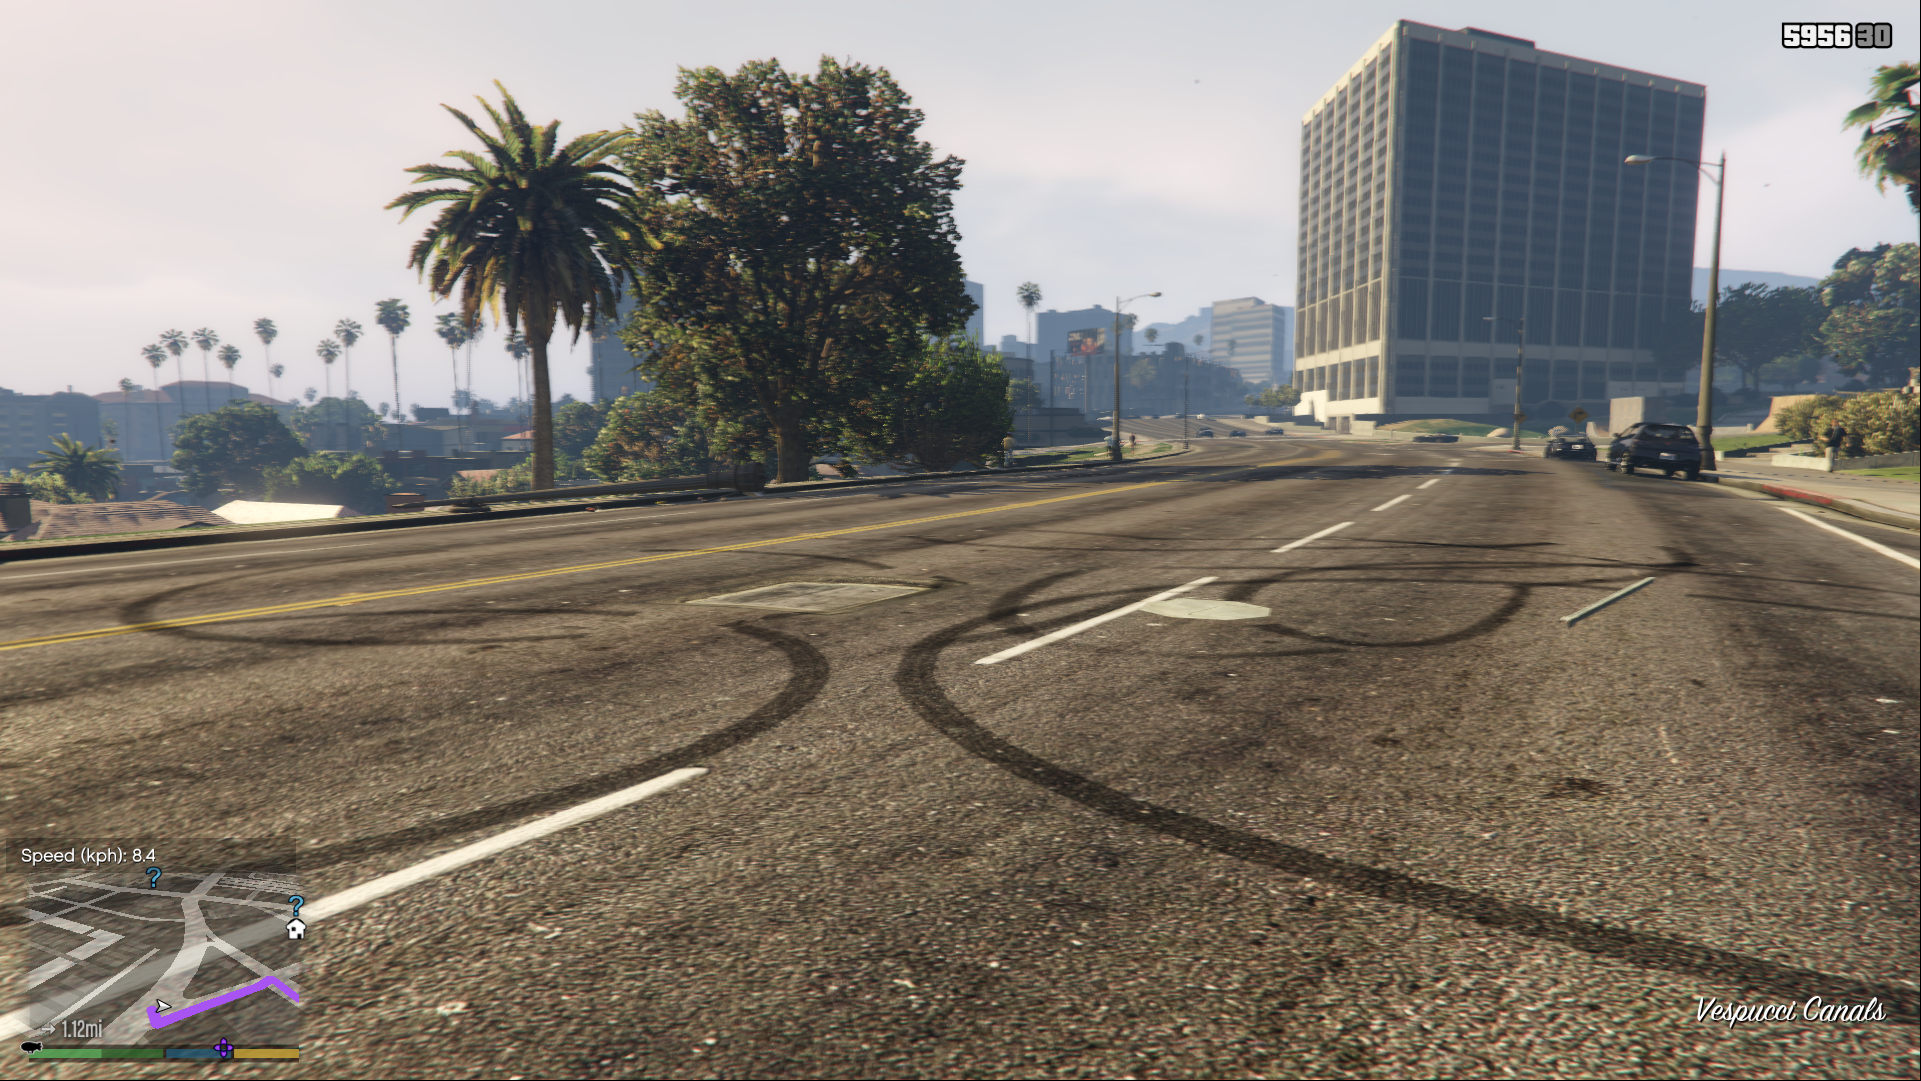
\includegraphics[width = 4in]{Ch03/0000001.png}
    \caption{Recorded Image}
    \label{figure:1}
\end{figure}

\subsection{Labels}
The dataset comprises of four labels:
\begin{itemize}
    \item \textbf{\textit{Throttle Value}} is the value of the acceleration the car is in. Throttle value 1.0 means forward acceleration, 0.0 means backward acceleration and 0.5 means no acceleration.
    \item \textbf{\textit{Throttle Flag}} is a boolean value which states whether there is an acceleration.
    \item \textbf{\textit{Steering Value}} is the value of the steering of the car. Steering value 1.0 means left steering, 0.0 means right steering and 0.5 means no steering.
    \item \textbf{\textit{Steering Flag}} is a boolean value which states whether there is an steering.
\end{itemize}

\section{Data Preprocessing}

\subsection{Generating Navigation Map}
The Navigation System inbuilt in the game is extracted from the recorded image for coordinates (28,873) to (300,1045). Then since only the purple region is required to give the  path, it is colored white ann the rest part is colored black. Then the image is resized to 128 X 128.

\subsection{Generating Speed Map}
Using a modification in GTA-V, it is possible to have a digital speedometer which is just above the Navigation Map. From there, the speed is cropped from (125,843) to (173,869). Then the image is made binary. Then the extracted image is resized to 128 X 128.

\subsection{Resizing Image}
Since the map and speed is extracted from the original image, the region in image containing map and speed is masked to not contail it in the image. The region masked is from (20,839) to (300,1060). Then the image is resized to 256 X 256 to make the image computationally feasible for Neaural Network training. 
//
Figure 3.2 shows the processed images, map, speed.

\subsection{Collecting generate images and labels}
Then the processed images and map are pushed into a array and all the hence genrated array are pushed into another array to form training images named Xtrain and all the labels are pushed into another array to form training labels named Ytrain. Then the generated Xtrain and Ytrain are saved in .npz files.

\begin{figure}[h]
    \centering
    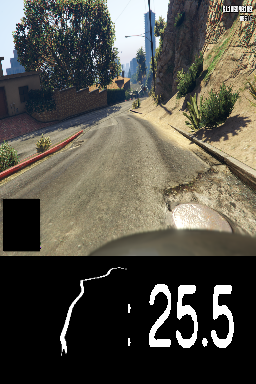
\includegraphics[width = 3in]{Ch03/final.png}
    \caption{Processed Images}
    \label{figure:2}
\end{figure}

\section{Model Designing}

\subsection{Creating Patches of Images}

\subsection{Transformer Encoder}

\subsection{Model Decoder}

\subsection{Final Model}